\documentclass[11pt]{article}
\usepackage[T1]{fontenc}
\usepackage{lmodern,amsmath,amssymb,xcolor,graphicx}
\usepackage[a4paper,margin=22mm]{geometry}
\usepackage[hidelinks]{hyperref}
\definecolor{Teal}{HTML}{007568}
\definecolor{Ink}{HTML}{172F40}
\renewcommand{\familydefault}{\sfdefault}
\setlength{\parindent}{0pt}
\setlength{\parskip}{.6em}
\newcounter{talkslide}
\newcommand{\slide}[5]{%
  \stepcounter{talkslide}%
  \ifnum\value{talkslide}>1\relax\clearpage\fi
  {\color{Teal}\bfseries SLIDE \thetalkslide\hfill #1}\par
  {\color{Ink}\large\bfseries #2}\par #5\par
  \vfill
  {\centering\setlength{\fboxsep}{0pt}\fcolorbox{Ink!18}{white}{\includegraphics[width=.98\linewidth,page=\thetalkslide]{presentation.pdf}}\par}
  \medskip{\footnotesize\color{Ink!78}#3\par}}
\begin{document}
{\huge\bfseries Speaker notes}\par
Constructive and Destructive Training Regimes\hfill 45-minute talk\par
\smallskip\hrule\medskip
% Each slide has a clock interval, title, evidence credit, projected content, and speaking notes.
\slide{00:00--01:00}{How much of a training step survives?}{}
{\displaylineoftext{Constructive and Destructive\\Training Regimes}
\vspace{1mm}\lead{From Gradient Interactions to Functional Oscillations}
\vspace{7mm}\point{How much of a training step survives the next one?}
\vspace{7mm}\par\small Thiago Mattar, Cristiano L. Castro, Frederico Coelho,\\ Yan G. Ferreira, and Antonio P. Braga}
{Open with a question. Suppose we watch a network make 50 updates. Its predictions change each time. If we put the first and last predictions side by side, how different do we expect them to look? Give the room a few seconds. In the spike windows we examined, the final difference was only a few percent of the distance the predictions had traveled. Yet the loss could still improve. The talk follows that puzzle from a single adjustable weight to the internal responses of an image or language model. We will end by changing how an optimizer acts on those responses.}

\slide{01:00--03:00}{What changes when a network learns?}{Paper, Sections I and III}
{\splitview{\point{From an image to a prediction}\par An image enters the network. Each layer produces a set of numbers, its \textbf{activations}. The output assigns scores to possible labels.}
{\point{From an error to an update}\par A \textbf{loss} scores how poorly the prediction fits the label. The \textbf{gradient} measures how sensitive that loss is to each weight.}
\vspace{5mm}\lead{Plain gradient descent (GD) moves the weights against the gradient. The learning rate sets the step size.}}
{Use the example of an image labeled cat. A classifier can already predict cat and still change how confidently it favors that label over dog. Loss can therefore move even when the winning label stays the same. Explain a weight as an adjustable number reused across many inputs. If there are a million weights, the gradient has a million components. Its direction points uphill locally, so plain gradient descent takes a step in the opposite direction. The optimizer then evaluates a new gradient at the new weights. Invite the audience to imagine that an update carries the weight past the best value for a feature. From the other side, the slope points back. This sets up the distinction between the direction of one step and the trajectory over many steps.}

\slide{03:00--05:00}{Four updates can leave very little displacement}{Illustrative example \(\cdot\) Paper, Section III}
{\lead{Imagine these changes to a single weight.}\vspace{2mm}
\[
        0 \;\xrightarrow{+1.0}\; 1.0 \;\xrightarrow{-0.9}\; 0.1
          \;\xrightarrow{+1.0}\; 1.1 \;\xrightarrow{-0.9}\; 0.2
\]
\splitview{\point{Total distance traveled}\par \(1.0+0.9+1.0+0.9=3.8\)}
{\point{Distance from the start}\par \(\lvert 0.2-0\rvert=0.2\)}
\vspace{4mm}\lead{The weight retains \(\boldsymbol{0.2/3.8\approx 5.3\%}\) of its path as net displacement.}}
{Read the sequence out loud before revealing the arithmetic verbally. Ask the audience to point at which updates undo the preceding one. All three adjacent pairs oppose each other, yet the final weight differs from the starting value. Lift the example into many dimensions: add the update vectors first and measure the length of their sum for displacement, or sum their individual lengths for distance traveled. The ratio measures cancellation and turning along the path. A curved path can also produce low retention, so later we will look for direct evidence of reversal. A small ratio alone tells us nothing about the value of the endpoint for the task.}

\slide{05:00--07:00}{A reversal can still bring the weight closer to the minimum}{Exact illustration \(\cdot\) \(L(w)=w^2/2\), \(w_0=1\)}
{\chart{quadratic}
\point{At learning rate 1.8, the weight crosses zero at every step while the loss decreases.}}
{The minimum of this one-weight loss is at zero. Its gradient is just the current weight, so the update is \(w_{t+1}=(1-\eta)w_t\). Work through the orange line: one becomes minus 0.8, which becomes plus 0.64. The endpoints alternate sides, yet the magnitude shrinks by a factor of 0.8 each time. The right plot measures squared distance to zero up to a constant, so it falls. Compare the teal line, which stays on one side. Pause on the distinction between oscillating weights and oscillating loss. This simple example has the former alone. In a network, the loss can fluctuate as well.}

\slide{07:00--09:00}{Two gradients reveal how the slope changed}{Paper, Section III and Appendix A}
{\(\rho_t=\cos(g_{t-1},g_t)\) compares successive gradients.
\par\point{Constructive regime}\enspace \(\rho_t>0\) \hfill
{\color{Rust}\bfseries Destructive regime}\enspace \(\rho_t<0\)
\vspace{3mm}
\[
   \eta\widehat\kappa_t
      =1-\rho_t\,\frac{\|g_t\|}{\|g_{t-1}\|}
\]
\lead{For smooth full-batch GD, this gives the average curvature along the completed step, scaled by the learning rate.}
\small On a quadratic loss, values above \(1\) imply reversal and values above \(2\) imply a loss increase on that step.}
{A cosine of one means the successive arrows point the same way. Minus one means they point opposite ways; zero means they are perpendicular. For plain GD, flipping the sign on both gradients to get the two steps leaves their cosine unchanged. Curvature describes how the slope changes as we travel. The equation needs a previous gradient, a current gradient, and two norms. For nonzero gradients the reversal threshold of one follows directly from the identity, even beyond a quadratic. For an on-the-board check, take a cosine of minus one. If the new norm is half the old one, the right-hand side is 1.5. If the new norm is twice as large, it becomes 3. Each step reverses, but only the second exceeds two. The threshold of two for the sign of the completed loss change is exact on a quadratic and has a remainder on a nonlinear loss. The largest Hessian eigenvalue describes the sharpest available direction. The measured value concerns the direction actually traveled.}

\slide{09:00--11:00}{The first experiment holds the training data fixed}{Paper, Section IV \(\cdot\) settings studied by Cohen et al., ICLR 2021}
{\begin{center}\renewcommand{\arraystretch}{1.3}
\begin{tabular}{@{}lll@{}}\toprule
Network & Prediction task & Data per GD update\\\midrule
MLP & Image label & 5,000 CIFAR-10 images\\
ResNet-32 & Image label & 50,000 CIFAR-10 images\\
Transformer & Next word & 59,680 WikiText-2 sequences\\\bottomrule
\end{tabular}\end{center}
\vspace{2mm}\lead{Within each model, three learning rates start from the same weights and run for 3,000 full-batch GD updates.}}
{The multilayer perceptron (MLP) is a small stack of fully connected layers. ResNet is a deeper image model with connections that let information skip across layers. The Transformer uses attention to predict words from earlier words. The losses have different units across these tasks; the comparisons that matter are within each model. Full batch means every update uses the entire chosen training objective. This rules out changing the sampled data as the explanation for any oscillations we see here. The setups connect to Edge-of-Stability work, which found that neural networks can continue to train near a classical curvature threshold. Ask whether two gradients can reveal when those dynamics begin.}

\slide{11:00--13:00}{The step-direction estimate approaches two}{Paper, Fig. 1 \(\cdot\) CIFAR-10 / MLP}
{\chart{gd-curvature}
\point{The higher-rate run keeps reducing loss overall. Its measured step curvature and its sharpest curvature follow different trajectories.}}
{Start with the left panel. The two curves use the same weights at initialization and the same examples. Follow the higher-rate curve beyond its initial transient. Its envelope continues downward even as successive loss values fluctuate. Both curves on the right belong to that higher-rate run. The orange curve is computed from training gradients. The dashed blue curve uses the largest Hessian eigenvalue, which requires extra derivative work. The dotted line is the quadratic reference value of two. The plotted curvature curves are centered 101-step means; sharpness was measured every 100 updates and interpolated. These averages describe a training regime. They cannot be used retrospectively as a per-step warning test.}

\slide{13:00--15:00}{Larger steps can repeatedly undo earlier steps}{Paper, Fig. 2 \(\cdot\) CIFAR-10 / MLP at \(\eta=0.04\)}
{\chart{gd-reversal}
\point{After 3,000 updates at the highest rates, net displacement is 2.6\%, 3.7\%, and 5.4\% of path length for MLP, ResNet, and Transformer.}}
{The left panel now measures alignment. When the curve approaches minus one, the new gradient largely opposes the previous one. The right panel measures the gradient's length. With a fixed learning rate, longer gradients mean larger steps. The 50-observation trailing averages make the regime visible. Put those observations together: the network takes substantial steps, then partly retraces them. Recall the four-step arithmetic. Across all three high-rate runs, the endpoint retains only a few percent of the parameter path. Each of these rates nevertheless gives the lowest final training loss for its model among the three tested. This is inefficiency in translating travel into displacement. A representation-learning interpretation is that later updates may interfere with structure that earlier updates built. To test that possibility, we will measure responses to the same inputs; the parameter curves alone do not establish forgetting.}

\slide{15:00--17:00}{The reversal recurs beyond the preceding step}{Paper, Fig. 3 \(\cdot\) MLP, one fixed endpoint, highest tested rate}
{\chart{backward}
\point{Looking back one update gives an almost opposite gradient. Looking back two gives almost the same direction.}}
{Explain the horizontal axis before interpreting the plot. Choose the gradient after 2,256 plain GD updates and hold it fixed. The first point compares it to the gradient one step earlier, and the next compares it to the gradient two steps earlier. The endpoint never advances across this figure. The first cosines are about minus 0.98 and plus 0.97. Let the audience predict the sign at lag three. The alternation initially persists and weakens, with a slower early decay in the Transformer. The paper follows lags to 256, where alignment can strengthen again. This fixed-endpoint observation establishes a recurring pattern in these trajectories, without a momentum term in the optimizer.}

\slide{17:00--19:00}{Smaller batches weaken both kinds of alignment}{Paper, Fig. 4 \(\cdot\) WikiText-2 / Transformer at \(\eta=0.1\)}
{\chart{sampling}
\point{Read from right to left. Sampling pushes both the early positive cosine and the later negative cosine toward zero in magnitude.}}
{Stochastic gradient descent (SGD) estimates the full gradient from a batch. Two estimates contain a shared signal and fluctuations due to the examples sampled. At a fixed state, if gradient norms concentrate, the noise in those norms attenuates the expected cosine. Along a moving trajectory that is a prediction, which we test. Start the 200-update continuations either at initialization or after 2,000 full-batch updates. Each sampled point averages eight sampling repetitions at one initialization; hollow points use full GD. On the Transformer the early mean goes from approximately one to minus 0.09 at eight sequences. The late mean goes from minus 0.97 to minus 0.26. ResNet preserves intact BatchNorm groups, so its minimum is 1,000 images. Consequences for implicit regularization remain open.}

\slide{19:00--21:00}{Adam can switch regimes around a loss spike}{Paper, Fig. 5 \(\cdot\) ResNet-32, full-batch Adam at \(\eta=0.003\)}
{\chart{adam}
\point{Adam combines recent gradients and rescales each coordinate. Its applied step can point away from the raw gradient direction.}}
{Start with the left plot of a full-batch Adam run. Even with identical training data every step, sharp excursions recur. On the right, zoom in on the raw-gradient alignment during the shaded interval. Locate the loss peak, then identify a period of constructive alignment in the recovery. Here the gradient norm grows on the approach to the spike. In the paper, raw gradients are evaluated before Adam applies each new update. This lets us ask whether the most recent response is informative about the next loss. This differs from the persistent destructive regime in high-rate GD. To see why Adam can behave differently, imagine a coordinate that has seen large gradients for several updates. Adam keeps a running average of squared gradients, which rescales the proposal for that coordinate. It also averages gradient directions over time. For a general optimizer, projecting the full gradient difference onto the actual step \(u\) and dividing by \(\|u\|^2\) recovers the exact path-average curvature on a smooth fixed loss. Adam's raw-gradient diagnostic projects onto the preceding gradient instead. That distinction makes its predictive value an empirical question.}

\slide{21:00--23:00}{Can the last two gradients warn about the next step?}{Paper, Section V \(\cdot\) 1,023 decisions per full-batch Adam trajectory}
{\small Issue a warning before the next update if
\(1-\rho_t\|g_t\|/\|g_{t-1}\|>2\).
The target is a \(\geq 0.1\%\) increase in loss on the next step.
\begin{center}\renewcommand{\arraystretch}{1.24}
\begin{tabular}{@{}lrrr@{}}\toprule
& MLP & ResNet & Transformer\\\midrule
Usual chance of a rise & 43.6\% & 8.6\% & 13.9\%\\
Chance after a warning & 55.8\% & 58.3\% & 53.7\%\\
\textbf{Warning lift} & \textbf{1.28\(\times\)} & \textbf{6.78\(\times\)} & \textbf{3.87\(\times\)}\\\bottomrule
\end{tabular}\end{center}
\point{On ResNet, an increase followed about 58 of every 100 warnings.}}
{Distinguish three clocks. The gradients are available now; their difference describes the preceding step; the decision concerns the outgoing Adam update. The rule is simply a threshold, without a trained classifier. The table's event is a one-step rise of at least 0.1 percent, which is much smaller than the excursions we select for tracing. Explain the middle column by imagining a hundred randomly selected ResNet steps: roughly nine raise loss this much. Among a hundred warnings about 58 would do so. Dividing these probabilities gives the lift. The combined condition had the highest lift and accuracy among the rules tested, including a warning when the previous loss rose. There are still many false alarms. We did not use this warning to trigger the intervention in the reported experiments.}

\slide{23:00--25:00}{How do we measure a change in the learned function?}{Paper, Section V \(\cdot\) illustrative two-input example}
{\lead{Show the \textbf{same inputs} before and after every update. Record a unit's response on each one.}
\begin{center}\renewcommand{\arraystretch}{1.2}
\begin{tabular}{@{}lrrr@{}}\toprule
 & Before & After step 1 & After step 2\\\midrule
Input A & 1.0 & 1.4 & 1.1\\
Input B & 2.0 & 1.8 & 1.95\\\bottomrule
\end{tabular}\end{center}
\(\delta_1=(+0.4,-0.2)\), \quad \(\delta_2=(-0.3,+0.15)\).
\par\point{Here the second change points exactly opposite to the first.}}
{Keep the reference inputs and their order fixed. Point out that the network's responses remain positive in this example. The reversal is in their changes. The second change is minus three quarters of the first, so the cosine between the two changes is minus one. In the real measurements the vector stacks every recorded feature at every matching position for one site. Its length measures the magnitude of the change; dividing by the square root of the number of coordinates gives a root-mean-square size. Its cosine with the preceding change measures functional alignment. The inputs are all 5,000 training images for the MLP, an intact group of 1,000 images for ResNet, and 64 complete sequences for the Transformer.}

\slide{25:00--27:00}{Outputs and early layers can move differently}{Paper, Fig. 6 \(\cdot\) ResNet spike trace, updates 390--450}
{\chart{hidden}
\point{Blue means reversal on the left. Bright yellow means large movement on the right. The dashed line marks the loss peak.}}
{Read one column vertically as a snapshot across depth, then read the output row from left to right. Blue in the output row means that the current change reverses its predecessor. Earlier layers can still show reinforcement at the same update. The right panel uses a different quantity: each site's RMS movement divided by its own maximum over this window. Bright cells locate the largest changes in time, without comparing their absolute magnitude across layers. The traced ResNet event was selected as the last recovered loss excursion above 100 percent before step 512 in its native continuation. The first displayed output reversal occurs at step 391, the 10 percent loss-rise marker is at 406, and the peak is at 415 in this separately traced ResNet run. The Transformer also reverses before the sharp rise; the MLP is already reversing when its window opens. Trace two updates on either side of the black line with a finger and ask whether all layers have matching colors. This makes the difference between the timing of a large change and the direction of that change visible. These are observations around one selected spike per model.}

\slide{27:00--29:00}{Only a small fraction of output movement survives}{Paper, Section V \(\cdot\) net displacement divided by total distance on fixed inputs}
{\begin{center}\renewcommand{\arraystretch}{1.4}
\begin{tabular}{@{}lrrr@{}}\toprule
Path retained & MLP & ResNet & Transformer\\\midrule
First measured site & 3.25\% & 3.72\% & 24.33\%\\
\textbf{Output} & \textbf{1.71\%} & \textbf{2.44\%} & \textbf{3.51\%}\\\bottomrule
\end{tabular}\end{center}
\vspace{4mm}\lead{For every 100 units the MLP predictions traveled, their endpoint lay about \point{1.7 units} from where they started.}}
{Return to the opening question. The numerator measures how different the predictions look if we keep only the first and last state. The denominator adds up the lengths of every intermediate change. Both are measured in the same vector of responses on the same inputs. A 1.71 percent ratio is meaningful even though the underlying distance has many coordinates. Ask the audience to compare the Transformer's first row and output row. Its embedding finishes farther from its start relative to its own travel. That does not imply that the embedding moved a greater absolute distance. Low retention plus the negative change cosines is stronger evidence of repeated cancellation than either statistic alone. Try a numerical comparison aloud: if the embedding and output had each traveled 100 units in their respective coordinates, their endpoint distances would be about 24 and 3.5 units. Actual path lengths differ. This illustrates both the value and the limit of normalization.}

\slide{29:00--31:00}{Does the network keep reversing the same change?}{Paper, Section V \(\cdot\) intuition for singular value decomposition}
{\lead{Suppose the observed changes on two inputs are}
\[
    (+2,-2),\qquad(-1,+1),\qquad(+3,-3).
\]
\lead{Every update is a signed multiple of the \textbf{same direction}. Two recorded coordinates contain just one direction of movement.}
\vspace{2mm}\point{Singular value decomposition (SVD) finds the direction capturing the most squared movement, then the next orthogonal direction, at each site.}}
{Ask how many directions are required to draw all three changes. A single line through the origin suffices; an update's signed position along it tells us magnitude and orientation. Rotate that line in thought. Once it no longer lines up with the observations, some movement is left unexplained. Singular value decomposition implements that fitting idea in many dimensions. Stack one flattened change per row of a matrix, with identical input and feature coordinates across rows. Right singular vectors describe recurring directions and the squared singular values rank how much movement each explains. The sign of a fitted vector is arbitrary, but whether two coefficients change sign is unaffected by that choice. This is what SVD adds beyond low retention: it tells us whether the same directions are being revisited.}

\slide{31:00--33:00}{Ten directions capture most of the movement}{Paper, Fig. 7a--c \(\cdot\) 51 MLP, 61 ResNet, and 49 Transformer updates}
{{\color{Teal}\fontsize{34}{38}\selectfont\bfseries 82--99\%}\par
\lead{of squared movement lies in the first ten directions at every measured site across the three spike windows.}
\vspace{3mm}
\splitview{\point{At the output}\par The first direction alone accounts for 53\% in the MLP, 27\% in ResNet, and 42\% in the Transformer.}
{\point{Across depth}\par Temporal overlap with the output rises from 0.46 at the Transformer embedding to 0.98 at its final block.}}
{Ten directions can explain most movement in a response vector containing many more coordinates. This is a window-specific statement about squared movement on fixed reference inputs. The decomposition has at most as many nonzero directions as there are observed updates, and the claim is about concentration even within that limit. Explain temporal overlap separately: two layers have different units and can have different widths, so we compare the time courses of their leading ten directions over the same updates. One means identical temporal subspaces. In ResNet, overlap rises from 0.57 at the first convolution to 0.99 at the last residual stage. Shared timing is compatible with propagation, but cannot identify which layer caused the oscillation.}

\slide{33:00--35:00}{Predictions reverse along their leading direction}{Paper, Fig. 7d--f \(\cdot\) one output direction fitted per model and spike window}
{\chart{output-direction}
\point{A sign change means the next update reverses its contribution along the same fitted pattern.}}
{The horizontal axis is a training update inside a spike window. The vertical axis is the signed projection of that update's output-change vector onto the leading direction, divided by the square root of its number of coordinates. It is a change per update, not the cumulative position of the network. Start in the ResNet panel: the large positive and negative excursions occur in a narrow interval. The numerical scales differ across the panels, so compare the sequences of signs rather than their absolute heights. A coefficient returning to zero means that one update has little component along this direction; the whole network need not have returned to a previous function. Together with retention, this plot motivates limiting the size of the largest functional changes.}

\slide{35:00--37:00}{Cap the response an Adam step would induce}{Paper, Section VI \(\cdot\) direct response of one selected unit}
{\lead{Take the proposed weight change for one unit. Apply it to that unit's fixed reference inputs to estimate its direct root-mean-square (RMS) response change \(s\).}
\[
       \Delta\theta_{\rm capped}
       =\min(1,\tau/s)\,\Delta\theta_{\rm Adam}
\]
\point{Example}\quad If \(s=0.12\) and the budget \(\tau=0.04\), apply one third of that unit's proposed update.
\par\small Other units receive their own scale factors.}
{RMS means square each response change, average across reference inputs, then take the square root. For a linear unit with reference input matrix \(H\), the direct changes are \(H\Delta\theta\), so the score is \(\|H\Delta\theta\|/\sqrt n\). This is a direct response with the inputs held fixed. Updates further upstream may alter those same inputs during the actual forward pass. The procedure is local and does not require an SVD during training. Adam computes its moments as usual. Each selected unit keeps its proposed parameter direction, but its magnitude is reduced when the score exceeds the site's budget. A zero score needs no scaling. Emphasize that the cap was motivated by functional observations and applied to selected hidden units.}

\slide{37:00--39:00}{How do we tell whether the cap helped?}{Paper, Section VI and matched-outcomes table}
{\splitview{\point{Start from the same training state}\par Match the weights, Adam moments, random state, and number of updates within each model. Compare with unchanged Adam.}
{\point{Change one intervention}\par Try three cap budgets, three lower learning rates, three lower second-moment coefficients, and two clipping thresholds.}
\vspace{5mm}\lead{Measure final loss, mean loss, and the sum of all upward loss changes.}}
{Calibrate each site's budget using the 25th, 50th, or 75th percentile of observed unit displacements in the eight Adam updates before treatment. q25 is therefore the tightest of the three. The selected sites are the MLP's hidden linear maps, ResNet's convolutions, and the Transformer's query, key, value and feed-forward projections. Explain the third metric with a short example: a loss path 1.0, 0.8, 0.9, 0.7 has upward variation 0.1. Unlike final loss, it records the upward excursion even though the run ultimately finishes lower. A very small learning rate might win on smoothness alone. Ask the audience to predict how it would look if it also slowed optimization. The continuations match update count; computing the cap adds time.}

\slide{39:00--41:00}{A smoother run can still finish at higher loss}{Paper, Fig. 8 \(\cdot\) selected ResNet continuations, relative to unchanged Adam}
{\chart{tradeoff}
\point{q25 improved both outcomes in every model. In ResNet, reducing the learning rate tenfold nearly eliminated upward variation but increased final loss.}}
{First locate the cross at one, one. Move left for lower final training loss, down for less total upward variation. Ask the audience to choose an intervention if they care only about avoiding upward motion. The point far to the right and low in the plot is the tenfold learning-rate reduction. It suppressed upward variation by about 99 percent, yet its final loss was 0.245 versus 0.0067 for unchanged Adam. The q25 cap reached 0.0049. Across all three models and all three budgets, the caps lowered mean loss and upward variation. The best mean-loss budget differed: q50 in MLP and Transformer, q25 in ResNet. A single setting does not win every metric.}

\slide{41:00--43:00}{The cap reduces how far predictions swing}{Paper, Fig. 9 and Section VI \(\cdot\) q25 versus unchanged Adam}
{\begin{center}\renewcommand{\arraystretch}{1.4}
\begin{tabular}{@{}lrrr@{}}\toprule
 & MLP & ResNet & Transformer\\\midrule
Reduction in largest RMS output change & 93\% & 33\% & 45\%\\
Updates with output reversal under q25 & 50\% & 60\% & 89\%\\\bottomrule
\end{tabular}\end{center}
\vspace{3mm}\lead{In the Transformer, nearly nine in ten updates still reverse, even though the largest output change falls by \point{45\%}.}}
{Read the first row as a comparison of two maxima over matched continuations, one with and one without the cap. Read the second as the fraction of updates in the capped continuation whose output-change vector has negative cosine with the preceding vector. The denominators are different; these are answers to two separate questions. The cap made reversals smaller while they remained common. Distinguish this experiment from clipping the norm of the entire raw gradient. The cap acts on the direct response implied by an individual unit's proposed Adam increment. Measuring these unit responses adds computation. A lower loss after a fixed update budget does not establish a lower time to the same loss.}

\slide{43:00--45:00}{What should an optimizer try to preserve?}{Paper, Section VII \(\cdot\) discussion}
{\lead{A destructive regime can coexist with learning progress. During the measured spikes, predictions repeatedly reversed in a low-dimensional functional subspace.}
\vspace{3mm}\lead{Limiting large hidden-unit responses reduced the size of those swings and lowered mean training loss across all three models.}
\par\small Evidence comes from three models, selected spike windows, and primarily full-batch training.\par\vspace{2mm}\normalsize\point{Next experiment}\quad Use the inexpensive gradient warning to trigger the more costly cap. Compare both loss and elapsed training time.}
{Close by answering the opening question at both levels. Many parameter steps can cancel. Around these selected spikes, only 1.7 to 3.5 percent of the output journey remains as net displacement. Observing that behavior led to a concrete decision about which updates to shrink. The strongest limits are the modest model sizes, one initialization per model for the main comparisons, selected spike windows, and predominantly full-batch experiments. The cap continuations measure training loss over a fixed horizon. They do not establish improved generalization. How these results extend to large-scale mini-batch training and held-out performance is open. A warning-triggered cap is a proposal, not a result. Other future comparisons could encourage compact representations or recruit persistently inactive units. End by asking which test would show that an optimizer improved learning per unit of compute. Leave the slide up for questions.}

\clearpage
{\LARGE\bfseries Technical questions}\par
\textbf{Why does the diagnostic extend to any optimizer?}
For a nonzero applied step \(u=\theta_t-\theta_{t-1}\) and full gradients of a fixed, twice continuously differentiable loss, integrating the gradient along the step gives
\[
\frac{u^\top(g_t-g_{t-1})}{\|u\|^2}
=\int_0^1\frac{u^\top H(\theta_{t-1}+au)u}{\|u\|^2}\,da.
\]
The right side is the exact average directional curvature. If the Hessian is \(L_H\)-Lipschitz along the step, the discrepancy from the starting-point curvature is at most \(L_H\|u\|/2\). Substituting \(u=-\eta g_{t-1}\) recovers the GD diagnostic on slide 5. With Adam, use the actual increment to recover this curvature. Sampling adds a projected gradient-noise difference. See manuscript Appendix A.

\textbf{Can a small retention ratio arise without reversals?}
Yes. With \(T\) equal, mutually orthogonal steps, net displacement grows as \(\sqrt{T}\) while travel grows as \(T\). The ratio is \(1/\sqrt{T}\). This is why the measurements include adjacent cosines and the signed functional projections in addition to retention.

\textbf{What are the singular directions and the temporal overlap?}
At site \(\ell\), stack response changes as the rows of \(D_\ell=U_\ell\Sigma_\ell V_\ell^\top\).
A column of \(V_\ell\) is a direction across fixed input and feature coordinates. The fraction of squared movement in the first \(k\) directions is
\(E_k^\ell=\sum_{j\le k}\sigma_{\ell,j}^2/\sum_j\sigma_{\ell,j}^2\).
For \(k=10\), compute \(\|U_{\ell,k}^\top U_{\mathrm{out},k}\|_{\rm F}^2/k\).
Both temporal bases refer to the same updates, even when their sites have different widths. The Frobenius norm squares and sums all entries.

\textbf{Which related results motivate the study?}
Cohen et al., \emph{Gradient Descent on Neural Networks Typically Occurs at the Edge of Stability} (ICLR 2021), motivates the full-batch settings. Kingma and Ba, \emph{Adam: A Method for Stochastic Optimization} (2014), gives the adaptive update. Bai et al., \emph{Adaptive Preconditioners Trigger Loss Spikes in Adam} (ICML 2026), motivates the second-moment control. This study observes the gradient and functional response and directly tests a hidden-unit cap.
\end{document}
